\documentclass[11pt]{article}

\input{../../utils/preamble_problemas}
\xsimsetup{
solution/print = true
%solution/print = false
}

\title{Introducción a la física}
\author{Manuel Carlevaro}
\date{Universidad de Navarra}


\begin{document}
%\maketitle

\begin{center}
\framebox[1.0\textwidth][c]{
\huge{\textsc{Introducción a la física}} 
}
\end{center} 

\begin{center}
\vspace{1em}
\Large{\textsc{Universidad de Navarra}} 
\end{center}

 \vspace{1em}

\begin{center}
\begin{tabular}{r l}
 \textbf{Tema:} & Dinámica.\\
 \textbf{Profesor:} & Manuel Carlevaro \\
 \textbf{Ayudante:} & Alba Meneses Felipe
\end{tabular}\end{center}

\vspace{2em}

\begin{multicols}{2}
\begin{exercise}
    ¿Qué fuerza neta se requiere para impartir a un refrigerador de \qty{135}{kg} una aceleración de \qty{1.40}{m/s^2}?
\end{exercise}
\begin{solution}
    \qty{189}{N}
\end{solution}
\end{multicols}

\begin{multicols}{2}
\begin{exercise}
    Un carrito de juguete de \qty{4.50}{kg} sufre una aceleración en línea recta (el eje $x$). La gráfica muestra esta aceleración en función del tiempo. a) Calcule la fuerza neta máxima sobre este carrito. ¿Cuándo ocurre esta fuerza máxima? b) ¿En qué instantes la fuerza neta sobre el carrito es constante? c) ¿Cuándo la fuerza neta es igual a cero?
    \begin{center}
        \includegraphics[scale=0.45]{figs/prob-01.png}
    \end{center}
\end{exercise}
\begin{solution}
    a) \qty{45.0}{N}, b) entre los \qty{2.0}{s} y los \qty{4.0}{s}, c) a los \qty{0.0}{s} y a los \qty{6.0}{s}.
\end{solution}
\end{multicols}

\begin{multicols}{2}
\begin{exercise}
Un gato de \qty{2.75}{kg} se mueve en línea recta (el eje $x$). La figura muestra una gráfica de la componente $x$ de la velocidad de este gato en función del tiempo. a) Calcule la fuerza neta máxima sobre este gato. ¿Cuándo ocurre dicha fuerza? b) ¿Cuándo la fuerza neta sobre el gato es igual a cero? c) ¿Cuál es la fuerza neta en el tiempo \qty{8.5}{s}?
\begin{center}
    \includegraphics[scale=0.45]{figs/prob-02.png}
\end{center}
\end{exercise}
\begin{solution}
    a) \qty{11}{N}, entre los \qty{0.0}{s} y los \qty{2.0}{s}, b) entre los \qty{2.0}{s} y los \qty{6.0}{s}, c) \qty{2.75}{N}.
\end{solution}
\end{multicols}

\begin{multicols}{2}
\begin{exercise}
    En la superficie de Io, una luna de Júpiter, la aceleración debida a la gravedad es $g = \qty{1.81}{m/s^2}$. Una sandía pesa \qty{44.0}{N} en la superficie terrestre. a) ¿Qué masa tiene la sandía en la superficie terrestre? b) ¿Qué masa y peso tiene en la superficie de Io?
\end{exercise}
\begin{solution}
    a) \qty{4.49}{kg}, b) \qty{4.49}{kg} y \qty{8.12}{N}.
\end{solution}
\end{multicols}

\begin{multicols}{2}
\begin{exercise}
    Si la sandía del problema anterior se empujada por una fuerza horizontal neta de \qty{100.0}{N} en la superficie de Io, ¿cuál será su aceleración? ¿Y si fuera en la superficie terrestre?
\end{exercise}
\begin{solution}
    \qty{22.3}{m/s^2} en Io y en la Tierra.
\end{solution}
\end{multicols}

\begin{multicols}{2}
\begin{exercise}
    Un velero para hielo descansa en una superficie horizontal sin fricción. Sopla un viento constante (en la dirección de los patines del trineo), de modo que \qty{4.0}{s} después de soltarse el velero adquiere una velocidad de \qty{6.0}{m/s} ¿Qué fuerza constante ejerce el viento sobre el velero? La masa total del velero más el tripulante es de \qty{200}{kg}.
\end{exercise}
\begin{solution}
    \qty{300}{N}.
\end{solution}
\end{multicols}

\begin{multicols}{2}
\begin{exercise}
    Suponga que hay una fuerza de fricción horizontal constante con magnitud de \qty{100}{N} que se opone al movimiento del velero del problema anterior. En este caso, ¿qué fuerza debe ejercer el viento sobre el velero para producir la misma aceleración constante $a_x = \qty{1.5}{m/s^2}$?
\end{exercise}
\begin{solution}
    \qty{400}{N}.
\end{solution}
\end{multicols}

\begin{multicols}{2}
\begin{exercise}
    Dos adultos y un niño quieren empujar un carrito con ruedas en la dirección $x$ (ver figura). Los adultos empujan con fuerzas $F_1$ y $F_2$ como se muestra en la figura. a) Calcule la magnitud y dirección de la fuerza más pequeña que el niño debería ejercer para que el movimiento sea en dirección $x$ (despreciar los efectos de la fricción). b) Si el niño ejerce la fuerza mínima obtenida en el inciso a), el carrito acelerará a \qty{2.0}{m/s^2} en la dirección $+x$ ¿Cuánto pesa el carrito?
\begin{center}
    \includegraphics[scale=0.45]{figs/prob-03.png}
\end{center}
\end{exercise}
\begin{solution}
    a) \qty{-16.6}{N} $\hat{\bm{j}}$, b) \qty{839}{N}.
\end{solution}
\end{multicols}

\begin{multicols}{2}
\begin{exercise}
    Un jugador de baloncesto saltó una vez \qty{1.2}{m} sin carrera. (Esto significa que subió \qty{1.2}{m} después de que sus pies se separaron del piso.) El jugador pesaba \qty{890}{N}. a) ¿Qué rapidez tenía al separarse del piso? b) Si sus pies tardaron \qty{0.300}{s} en separarse del piso después de que inició su salto, ¿qué aceleración media (magnitud y dirección) tuvo mientras se estaba empujando contra el piso? c) Dibuje el diagrama de cuerpo libre. En términos de las fuerzas del diagrama, ¿qué fuerza neta actuó sobre el jugador? Use las leyes de Newton y los resultados del inciso b) para calcular la fuerza media que aplicó sobre el piso.
\end{exercise}
\begin{solution}
    a) \qty{2.42}{m/s}, b) \qty{8.07}{m/s^2} $\hat{\bm{j}}$, c) Fuerza neta \qty{733}{N} $\hat{\bm{j}}$, aplicó sobre el piso \qty{-733}{N} $\hat{\bm{j}}$. 
\end{solution}
\end{multicols}

\begin{multicols}{2}
\begin{exercise}
Una persona jala horizontalmente del bloque $B$ de la figura, haciendo que ambos bloques se muevan juntos como una unidad. Mientras este sistema se mueve, elabore un cuidadoso diagrama de cuerpo libre, rotulado, del bloque $A$, si a) la mesa no tiene fricción; y b)si  hay fricción entre el bloque $B$ y la mesa, y el tirón sobre el bloque $B$ es igual a la fuerza de fricción sobre él debido a la mesa.
\begin{center}
    \includegraphics[scale=0.45]{figs/prob-04.png}
\end{center}
\end{exercise}
\begin{solution}
    \begin{center}
        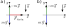
\includegraphics[scale=1.0]{figs/prob-05.pdf}
    \end{center}
\end{solution}
\end{multicols}

\begin{multicols}{2}
\begin{exercise}
    En una nave industrial una grúa (un gancho con una motor que enrolla y desenrolla una cuerda para subir y bajar objetos) sujeta una caja de \qty{200}{kg}. Dibuje un diagrama de cuerpo libre para la caja. Calcule la tensión en la cuerda si la caja a) sube a un ritmo constante; b) cuelga inmóvil de la cuerda; c) sube con aceleración de \qty{1.0}{m/s^2}; d) baja con aceleración \qty{1.0}{m/s^2}.
\end{exercise}
\begin{solution}
    a) \qty{1960}{N} $\hat{\bm{j}}$, b) \qty{1960}{N} $\hat{\bm{j}}$, c) \qty{2160}{N} $\hat{\bm{j}}$, d) \qty{1760}{N} $\hat{\bm{j}}$.
\begin{center}
    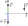
\includegraphics[scale=1.2]{figs/prob-06.pdf}
\end{center}
\end{solution}
\end{multicols}

\begin{multicols}{2}
\begin{exercise}
    Un elevador cargado, cuyos cables están muy desgastados, tiene masa total de \qty{2200}{kg}, y los cables aguantan una tensión máxima de \qty{28000}{N}. a) Dibuje el diagrama de cuerpo libre del elevador. En términos de las fuerzas de su diagrama, ¿qué fuerza neta actúa sobre el elevador? Aplique la segunda ley de Newton al elevador y calcule con qué aceleración máxima puede subir el elevador sin que se rompan los cables. b) ¿Cuál sería la respuesta al inciso a), si el elevador estuviera en la Luna, donde $g = \qty{1.62}{m/s^2}$?
\end{exercise}
\begin{solution}
    a) Si la aceleración es cero la fuerza neta es cero. La máxima aceleración de subida posible es \qty{2.93}{m/s^2}, b) En la luna la máxima aceleración de subida posible sería \qty{11.1}{m/s^2}. Diagrama de cuerpo libre identico al del problema anterior.
\end{solution}
\end{multicols}

\begin{multicols}{2}
\begin{exercise}
    Una mujer de \qty{50.0}{kg} se para en una balanza dentro un elevador. El elevador originalmente está bajando a \qty{10.0}{m/s}; pero se detiene con aceleración constante en una distancia de \qty{25.0}{m}. ¿Qué valor marca la balanza antes de comenzar a detenerse? ¿Qué valor marca la balanza mientras se está deteniendo?
\end{exercise}
\begin{solution}
    Antes de comenzar a detenerse marca \qty{50.0}{kg}. Mientras se está deteniendo marca \qty{60.2}{kg}.
\end{solution}
\end{multicols}

\begin{multicols}{2}
\begin{exercise}
    Un cubo es usado para tirar de un carro de sube por una pendiente (ver figura). El carro pesa \qty{50000}{N}. ¿Qué peso debe tener el cubo para que el sistema funcione con rapidez constante? Ignore la fricción en la polea y en las ruedas del carro, y el peso del cable.
\begin{center}
    \includegraphics[scale=0.5]{figs/prob-07.png}
\end{center}
\end{exercise}
\begin{solution}
    \qty{12947}{N}. 
\end{solution}
\end{multicols}

\begin{multicols}{2}
\begin{exercise}
La fuerza de fricción Ffric entre dos superficies se puede calcular fácilmente cuando están deslizando: $F_{\text{fric}} = \mu_d N$. Donde $N$ es la fuerza normal entre las superficies y $\mu_d$ es una constante que define la interacción de fricción dinámica (en deslizamiento, por eso el subíndice d). Por ejemplo, entre dos superficies de madera $\mu_d = 0.5$. ¿Con qué aceleración se deslizará un bloque de madera sobre una mesa de madera inclinada \ang{50} respecto de la horizontal?
\end{exercise}
\begin{solution}
    \qty{4.36}{m/s^2}.
\end{solution}
\end{multicols}

\begin{multicols}{2}
\begin{exercise}
    La fuerza de fricción $F_{\text{fric}}$ entre dos superficies no se puede calcular directamente cuando no están deslizando. Sólo sabemos que no puede superar un valor máximo: $F_{\text{fric}}^{\text{max}} = \mu_s N$. Donde $N$ es la fuerza normal entre las superficies y $\mu_s$ es una constante que define la interacción de fricción estática (sin deslizamiento, por eso el subíndice $s$ que significa \textit{static}).  Por ejemplo, entre dos superficies de madera $\mu_s = 0.6$ (El coeficiente estático es siempre mayor que el dinámico). Para saber la fuerza de fricción en un caso estático debemos deducirla de las otras fuerzas aplicadas a un cuerpo y del hecho de que el cuerpo no se mueve. ¿Cuál es la fuerza de fricción estática sobre un bloque de madera apoyado sobre una mesa de madera inclinada \ang{20} respecto de la horizontal?
\end{exercise}
\begin{solution}
    $\qty{3.35}{m/s^2} \, M$, donde $M$ es la masa del bloque de  madera.
\end{solution}
\end{multicols}

\begin{multicols}{2}
\begin{exercise}
    El bloque de madera de los problemas anteriores se pone sobre una mesa que se inclina a diferentes ángulos $\theta$ respecto de la horizontal. Indique en cuales de los siguientes casos se mueve, si se mueve aceleradamente y en cuales está estático: a) $\theta = \ang{25.704}$, b) $\theta = \ang{26.565}$, c) $\theta = \ang{27.654}$, d) $\theta = \ang{31.430}$. (Cuidado: puede haber más de una respuesta posible).
\end{exercise}
\begin{solution}
a) estático, b) estático (si comienza estático) o a velocidad constante (si comienza en movimiento), c) estático (si comienza estático) o a aceleración constante (si comienza en movimiento), d) a aceleración constante. 
\end{solution}
\end{multicols}

\end{document}
